\label{chap:arch}
\subsection{Hardware}

The processing power and wireless capability of the wireless sensor nodes are provided by an Atmel
ZigBit 900MHZ RF module. It contains an ATmega 1281V 8-bit microcontroller connected to an
AT86RF212 RF Transceiver via a SPI interface. The Atmega 1281V is an low power 8 bit microcontroller
that is connected to the onboard sensors of the node. In order to be able to transmit or secure the
data, the microcontroller will communicate with the RF Transceiver. The Transceiver controller is a very low power chip,
capable of sending data up to 6 km. Also, the Transceiver contains a security module compatible
with AES-128. It supports hardware encryption and decryption for AES 128 ECB, but but for the AES
128 CBC it is available only the hardware encryption.


\begin{figure}[ht] \centering
  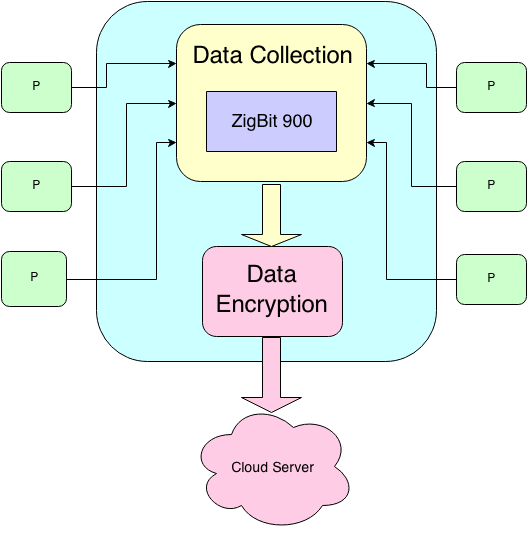
\includegraphics[width=0.5\textwidth]{img/wsn-soa-system-arch.png}
  \caption{System Architecture}
\end{figure}

\subsection{Software}

From the software perspective, the architecture is composed of three modules:
\begin{itemize}
\item data module, that
collects information from the sensors,
\item encryption module,
\item communication module.
\end{itemize}

The main focus on this paper will be placed on the encryption module.
The encryption method for the data uses the two supported hardware methods: AES 128 ECB
and AES 128 CBC. It is necessary to use both of them because the nodes are transmitting 
two kinds of packets: a first type of packets which contains non-sensitive data and is used by the
receiver to identify the sender and a second type of packets which contains the actual sensitive data. Since it supports 
both encryption and decryption, the first set of packets, those containing identification
information, are encrypted using ECB. The data itself is encrypted using CBC. Since CBC 
decryption is not supported by default, a software CBC decryption implementation is necessary in order to allow the sensors to verify the data at regular intervals.

 
%\begin{figure}[ht] \centering
%  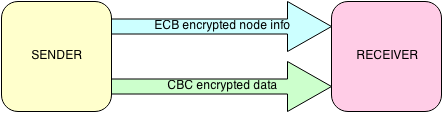
\includegraphics[width=0.5\textwidth]{img/send-receive.png}
%  \caption{Packet Types}
%\end{figure}


In addition to the CBC decryption, it is also required to have implementations of other software encryption algorithms in order to perform the performance analysis. The chosen 
algorithms which will be used in benchmarking are Skipjack and RC5.
